\section{Risk Mapping}
Our risk maps is constructed from three types of risk: poaching risk, wildfire risk, and tourism risk. Our maps are made over hexagons with sidelengths of around 3.1 km (so that the area, $\frac{3\sqrt{3}}{2}a^2$ is around 25 km$^2$; important for a later comparison to a square grid) through various data sources. We use hexagonal tessellation because it reduces edge effects and provides uniform adjacency compared to square grids \cite{birch2007hex}.

\subsection{Data Processing}

The raw-source provenance is tracked in \texttt{data/raw/manifest.csv}. For modeling, we collapse those inputs into a smaller set of derived spatial variables on a common Etosha hex grid. All geometries are clipped to the park boundary, projected to a metric CRS (EPSG:32733 \cite{epsg32733}) for distance and area calculations, and then aggregated to the grid. The grid itself is a flat-top hex lattice with target area $25$ km$^2$ per cell, which implies a side length of
\[
a = \sqrt{\frac{2A}{3\sqrt{3}}} \approx 3102 \text{ m}.
\]
Distance-based access variables are then built from cell centroids using exponential decay terms of the form $\exp(-d/\lambda)$, while wildlife and threat layers are rescaled to $[0,1]$ before combination.

\begin{table}[H]
\centering
\scriptsize
\begin{tabular}{p{0.18\textwidth} p{0.22\textwidth} p{0.18\textwidth} p{0.32\textwidth}}
\hline
\textbf{Raw source} & \textbf{Manifest entry / local artifact} & \textbf{Derived variables} & \textbf{Processing used in the model} \\
\hline
Park boundary and Etosha Pan & OSM/Nominatim boundary and pan exports \cite{osm} in \texttt{data/raw/etosha\_boundary/} & hex grid geometry, $d_{\mathrm{boundary}}$, $d_{\mathrm{pan}}$, pan overlap, terrain class & boundary polygon is used to clip the analysis extent; the pan polygon is intersected with each hexagon to compute pan-overlap ratio; cells are classified as pan, pan-margin, boundary-edge, or interior savanna from pan overlap and distance-to-boundary rules. \\

Road network & Geofabrik Namibia OSM shapefile extract \cite{geofabrik} (\texttt{roads}) & $d_{\mathrm{road}}$, tourist-road access, road access in poaching and tourism terms & roads are clipped to Etosha, tourist roads are handled as a designated subset, and centroid-to-network distances are converted into bounded access scores using exponential decay. \\

Waterholes, camps, and gates & Geofabrik POIs \cite{geofabrik} plus curated OSM-derived camp and gate tables \cite{osm} (\texttt{waterholes}, \texttt{camps}, \texttt{gates}) & $d_{\mathrm{waterhole}}$, $d_{\mathrm{camp}}$, $d_{\mathrm{gate}}$, tourism pressure inputs, poaching gate term, herbivore support input & point layers are cleaned and clipped to the park; centroid distances feed access surfaces and support layers. Gates and camps proxy human access and surveillance, while waterholes proxy both ecological aggregation and tourism concentration. \\

Elephants & GBIF occurrence pull \cite{gbif_elephant} (\texttt{elephants}) & elephant density support $E_i$ & point occurrences inside the boundary are converted to a smooth spatial density field by Gaussian KDE \cite{silverman1986kde} and then normalized to $[0,1]$ on the hex grid. \\

Lions & digitized ORC lion detections \cite{orc_carnivore} and GCP georeferencing files (\texttt{lion\_detections\_digitized}, \texttt{lion\_georeference\_gcps}) & lion support $L_i^{\mathrm{lion}}$ & approximate detections are georeferenced from the public figure, buffered by 10 km, unioned into support zones, clipped to the boundary, and erased from the pan; support then decays exponentially with distance from those zones and is normalized. \\

Rhinos & digitized Rhino Resource Center detections \cite{rrc_rhino} and GCP files (\texttt{rhino\_detections\_digitized}, \texttt{rhino\_georeference\_gcps}) & rhino support $Q_i$ and rhino-value term in poaching risk & approximate detections are georeferenced from the source figure, buffered by 6 km into a reference distribution, clipped to the boundary, and combined with distance-to-waterhole and pan-penalty terms; the resulting support field is normalized and reused directly in the poaching layer. \\

Wildfire history & NASA EONET wildfire events \cite{nasa_eonet} (\texttt{wildfires}) & historical fire-event count, recent-fire suppression $H_i$ & events intersecting each cell are counted; the wildfire model then converts any recent event into a suppression multiplier $H_i = 1 - 0.7\min(\text{count},1)$, reducing risk where recent burning likely lowered available fuel. \\

No direct raw layer; inferred ecological support & derived from waterhole distance, pan overlap, fire history, and terrain class & herbivore support $H_i^{\mathrm{herb}}$ & herbivore support is modeled rather than directly observed: water proximity raises support, pan overlap and recent fire reduce it, and terrain class contributes a multiplicative bonus or penalty. This gives a broad ungulate-support surface for the tourism and composite-risk calculations. \\
\hline
\end{tabular}
\caption{Raw spatial inputs, the model variables derived from them, and the main processing steps used before risk assembly. Table entries summarize the provenance recorded in \texttt{data/raw/manifest.csv} together with the transformation logic implemented in the preprocessing pipeline.}
\label{tab:risk_data_processing}
\end{table}

In practice, the data-processing pipeline has four layers. First, raw boundary, infrastructure, wildlife, and wildfire inputs are normalized into clean geospatial layers. Second, those layers are aggregated into per-cell geometric features such as centroid distances, pan overlap, and historical fire count. Third, wildlife support surfaces are built, using KDE for elephants, buffered digitized-reference zones for lions and rhinos, and a rule-based support proxy for herbivores. Fourth, the threat layers are computed from weighted combinations of those features, after which the species-by-threat tensor and composite map are assembled.


\subsection{Mapping Structure}
We built the risk heat maps on a hexagonal grid so the park could be divided into consistent spatial units. We used hexagons because each cell covers a comparable area and connects naturally to nearby cells \cite{birch2007hex}. That makes the maps easier to use later for movement, displacement, and resource allocation. It also gives a clearer spatial picture than treating risk as only a set of point locations.

Each hexagon is assigned wildlife support values and threat values. The wildlife side includes elephant density, rhino support, lion support, and herbivore support. The threat side includes poaching, wildfire, and tourism. All layers are normalized to the same scale so they can be combined directly. The main idea is that a hexagon should have high risk only when important wildlife presence overlaps with strong threat exposure.

\begin{figure}[H]
\centering
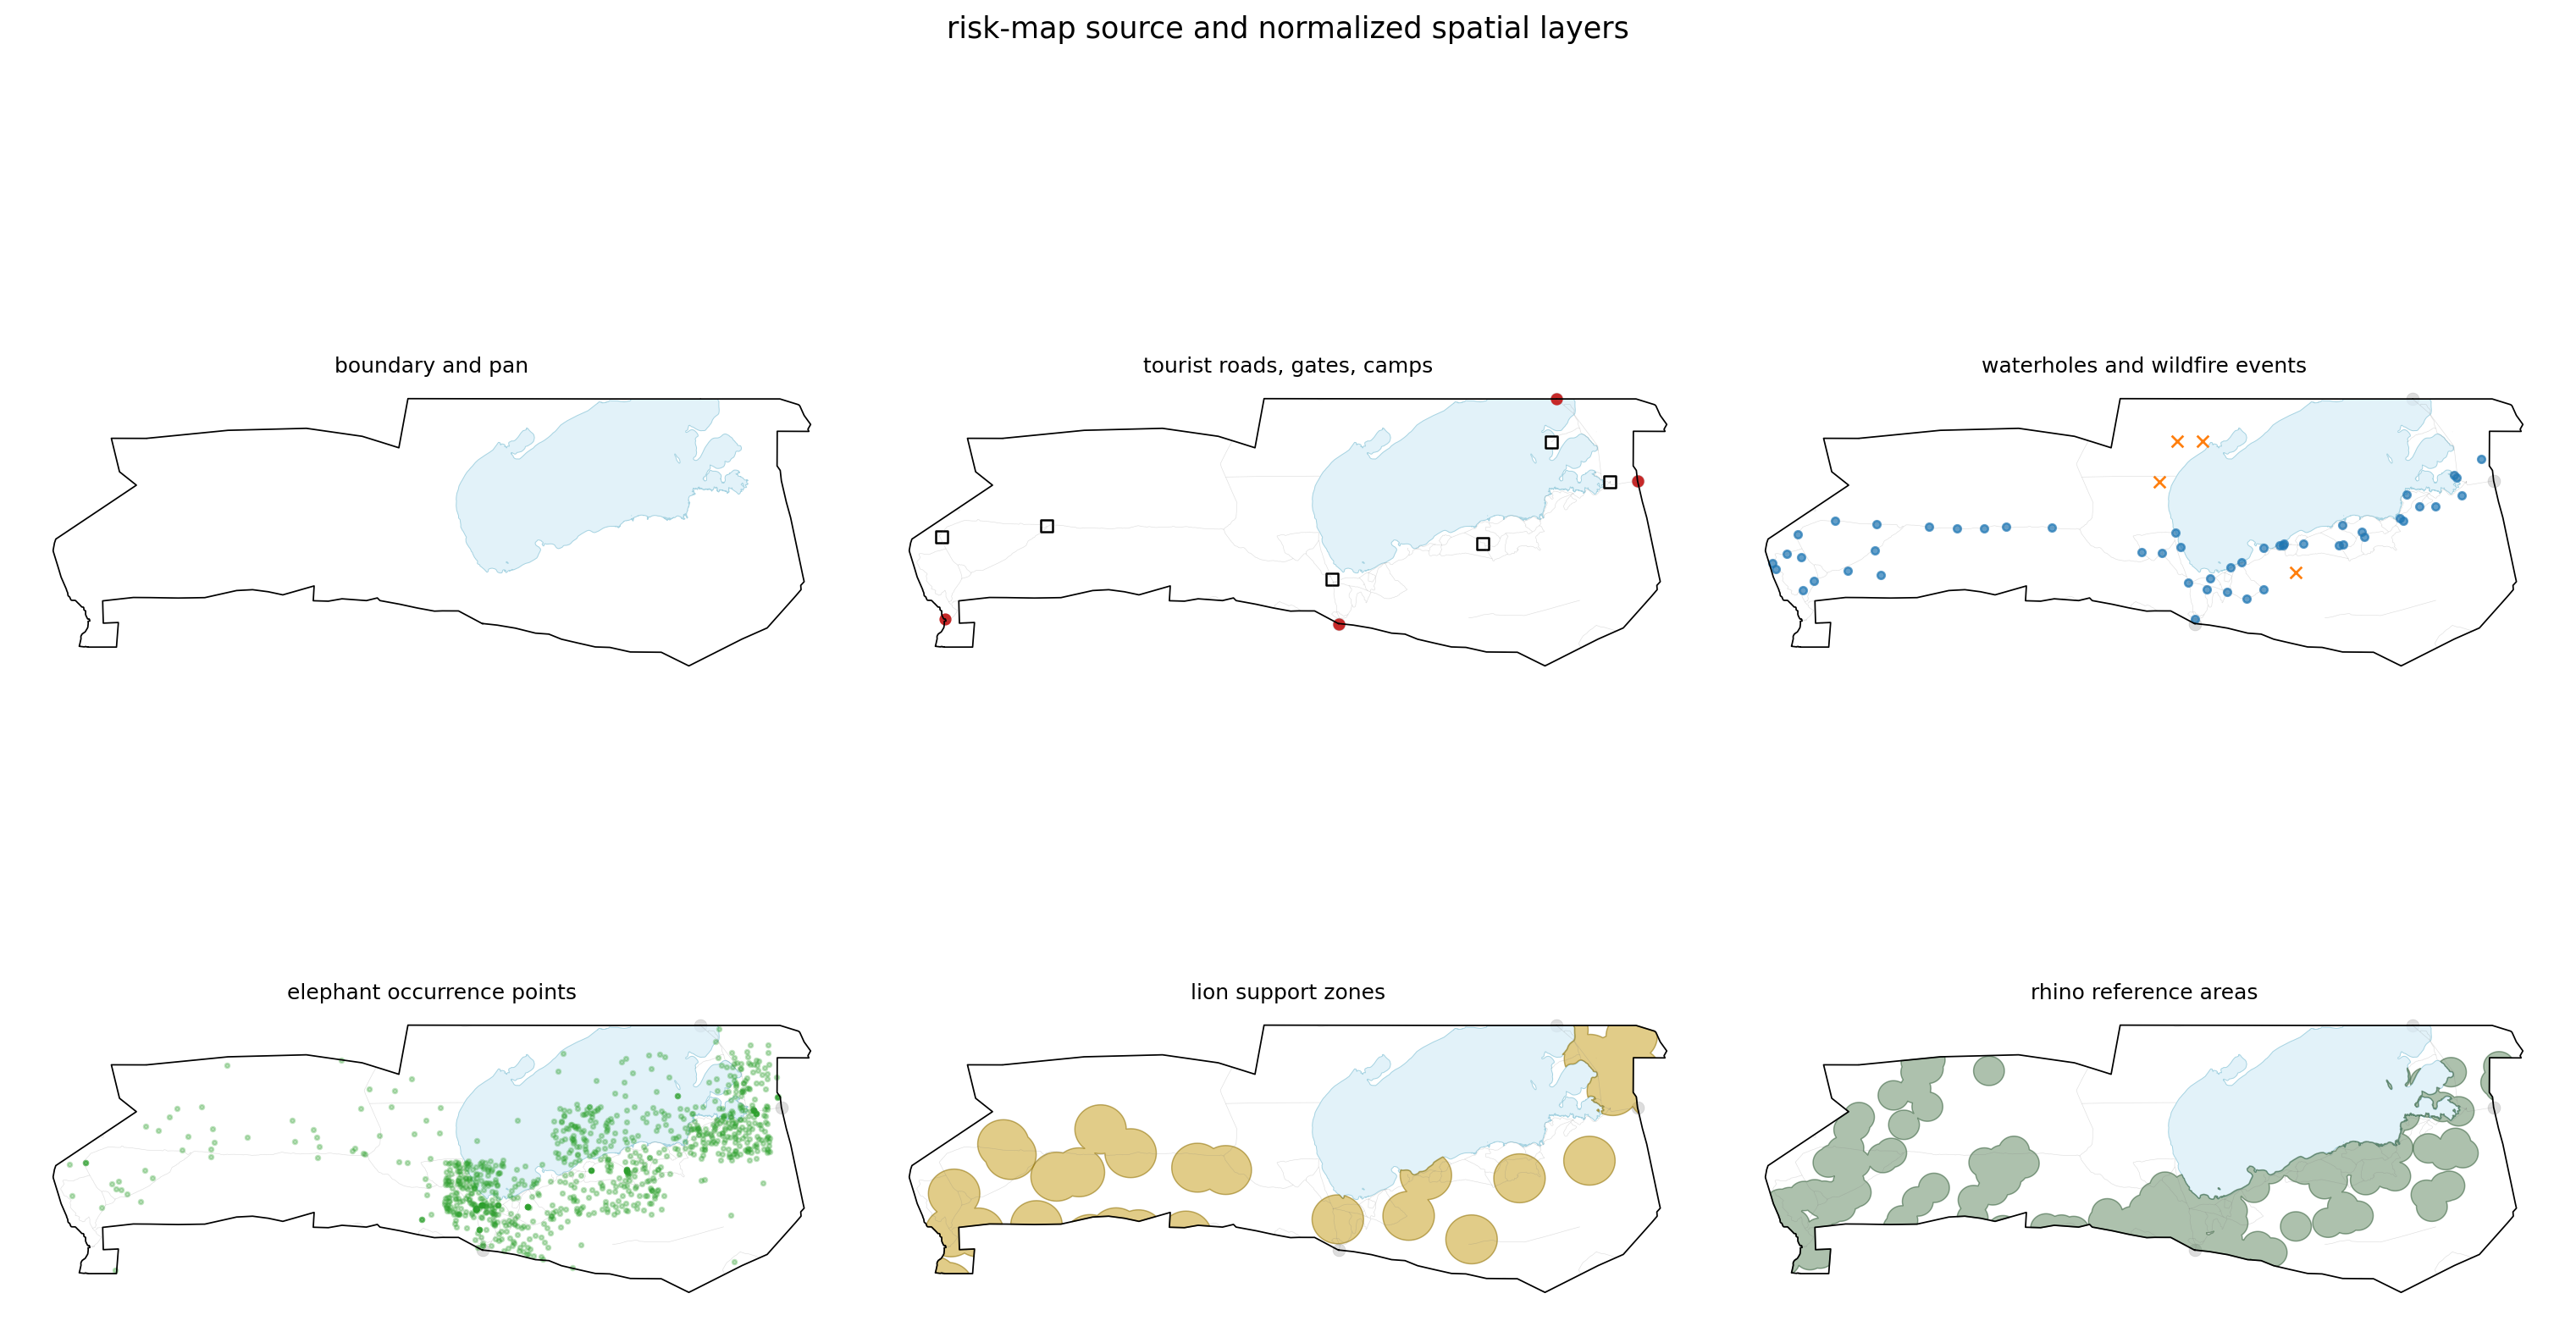
\includegraphics[width=0.95\textwidth]{risk_diagnostics/01_data_layers_overview.png}
\caption{Core spatial input layers used to construct the Etosha risk surfaces. These panels summarize the main environmental and access layers before wildlife support and threat-specific scoring are combined on the shared hexagonal grid.}
\label{fig:risk_data_layers}
\end{figure}

\begin{figure}[H]
\centering
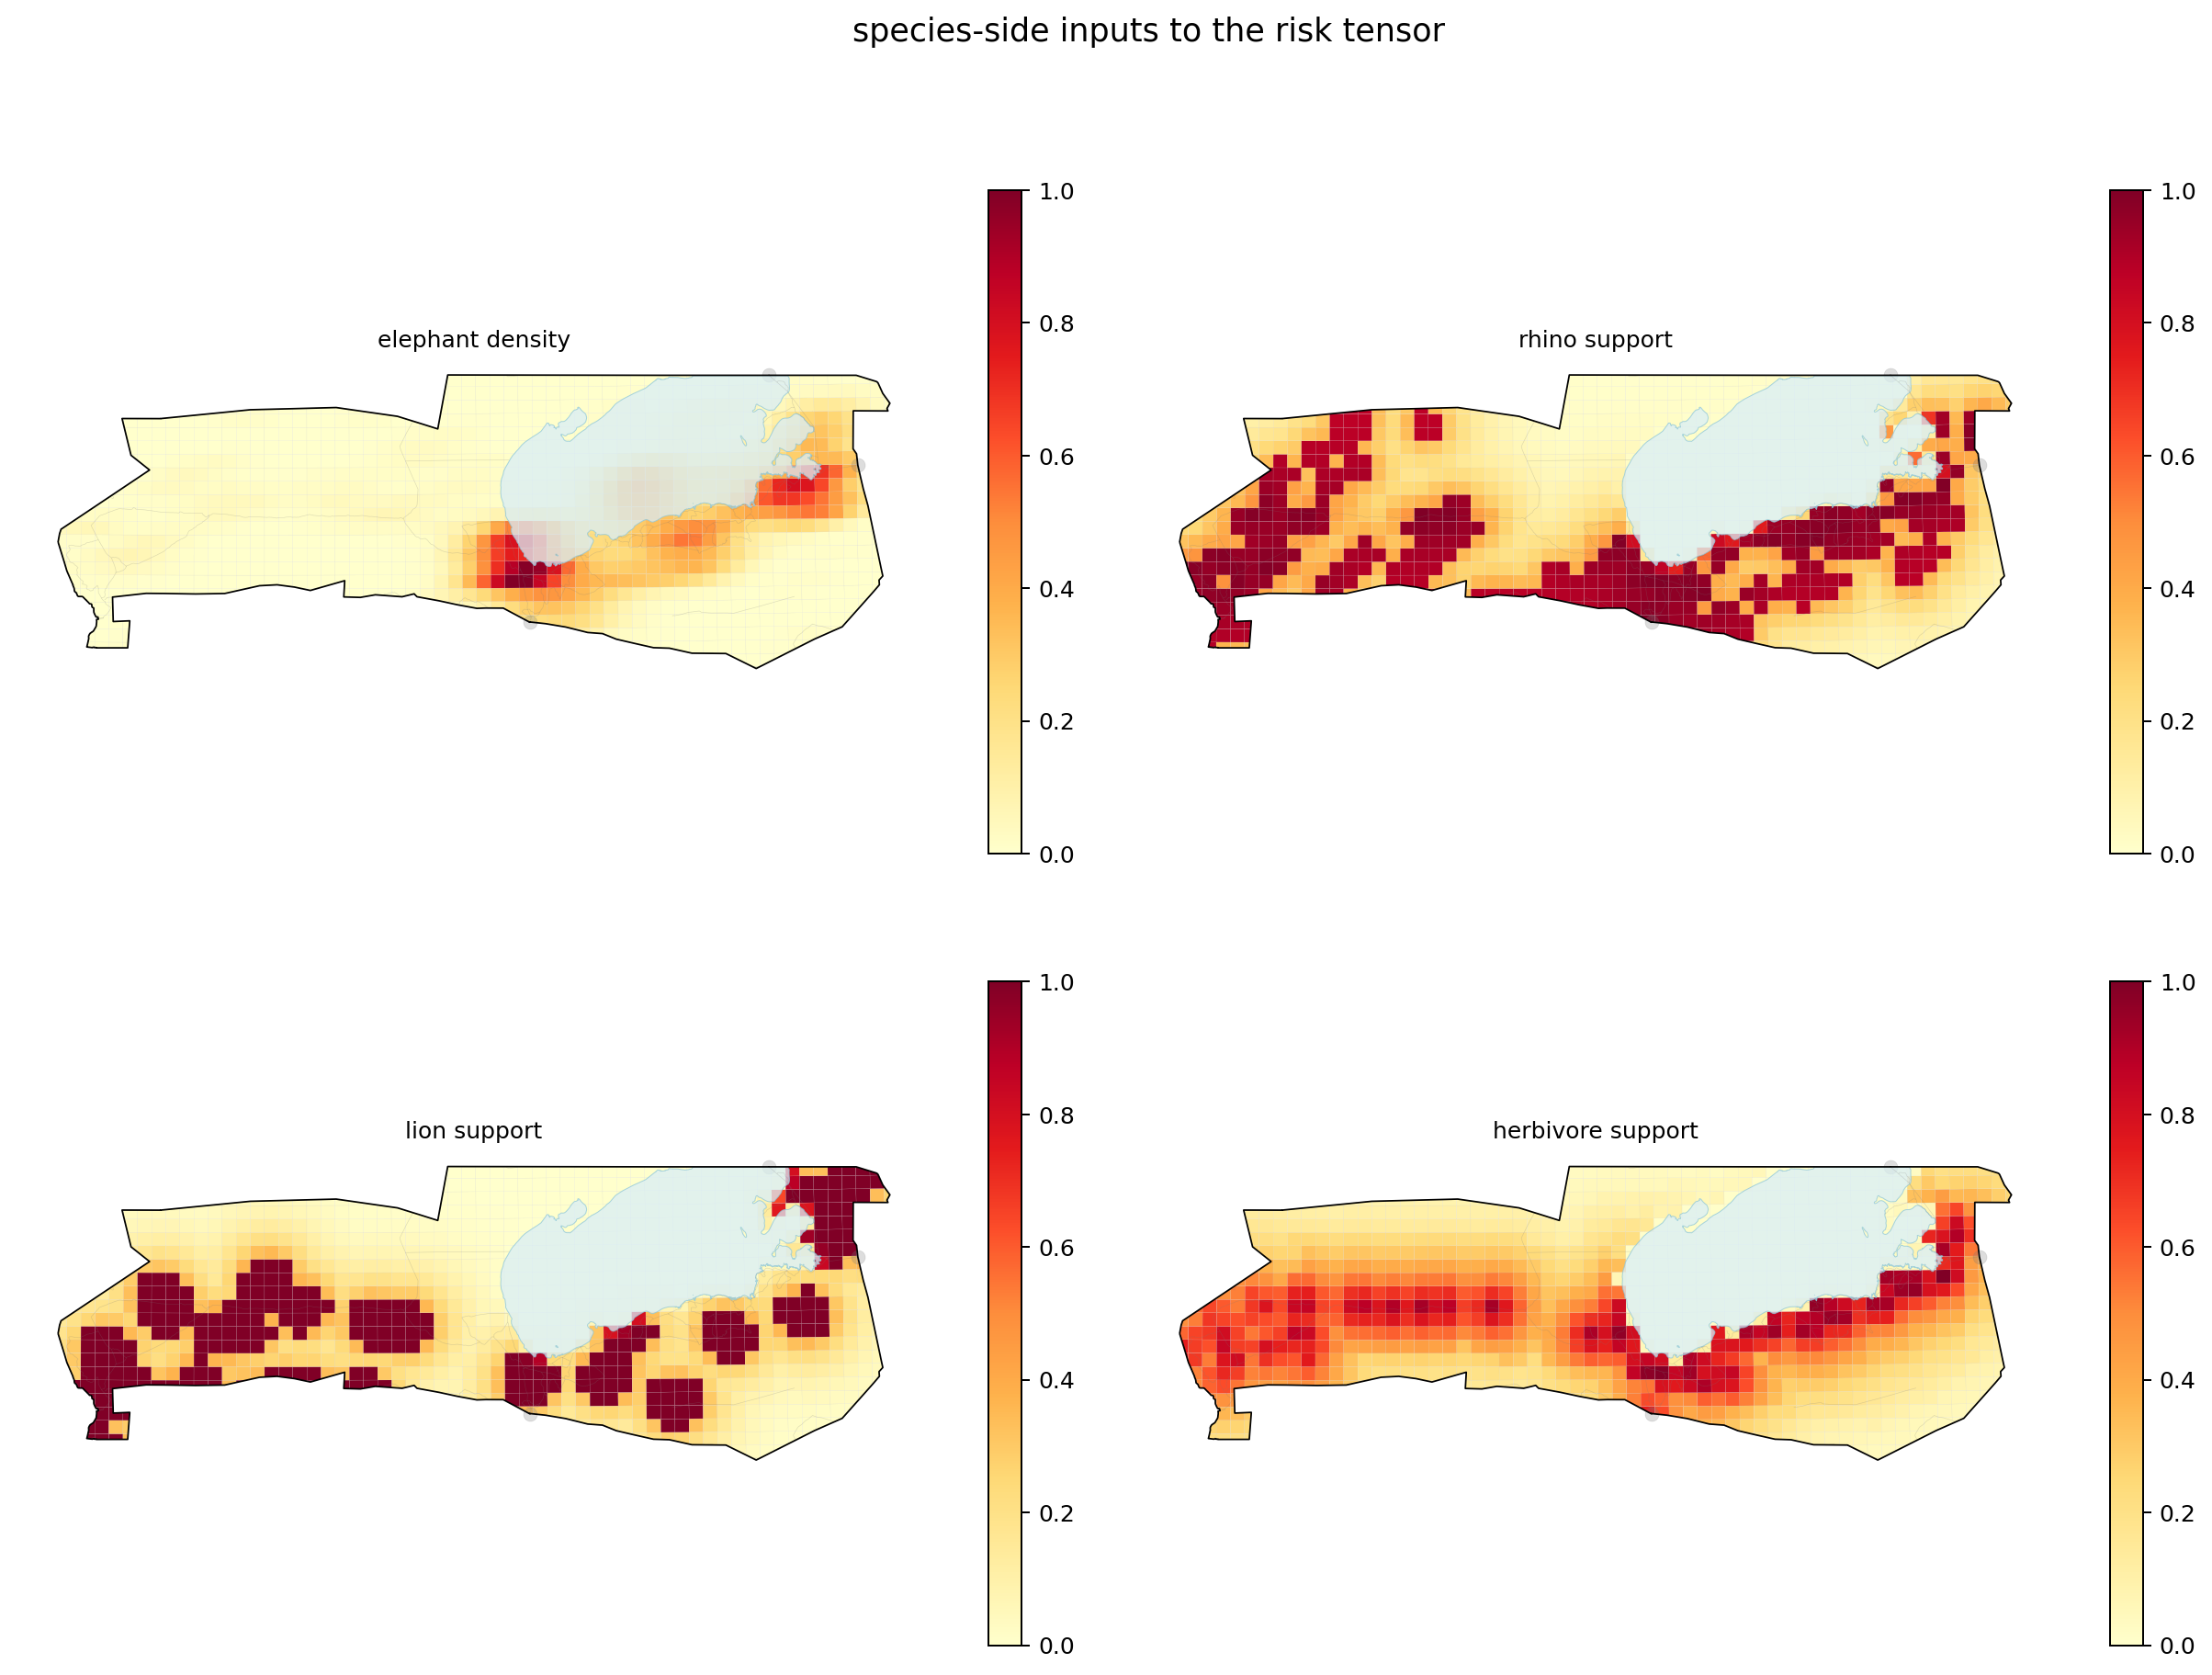
\includegraphics[width=0.95\textwidth]{risk_diagnostics/02_species_layers_overview.png}
\caption{Wildlife support layers on the same hexagonal lattice. Elephant, rhino, lion, and herbivore support are normalized and later combined with threat exposure so that species presence and hazard intensity enter the risk tensor on comparable scales.}
\label{fig:risk_species_layers}
\end{figure}

\subsection{Poaching Risk}
For poaching, the threat score is built from six parts: access from gates, access from the park boundary, access from roads, access from tourist roads, surveillance gaps, and rhino value. We define the poaching layer in hexagon $i$ by
\[
P_i
=
0.24\,G_i
+
0.24\,B_i
+
0.18\,R_i
+
0.08\,T_i
+
0.08\,S_i
+
0.18\,Q_i,
\]
where $G_i$ is gate access, $B_i$ is boundary access, $R_i$ is road access, $T_i$ is tourist-road access, $S_i$ is the surveillance-gap term, and $Q_i$ is rhino support. This places the greatest weight on locations that are easier to reach and especially valuable for rhino poaching, consistent with spatial poaching risk models that emphasize access and target value as primary drivers \cite{ferreira2015poaching}.

\begin{figure}[H]
\centering
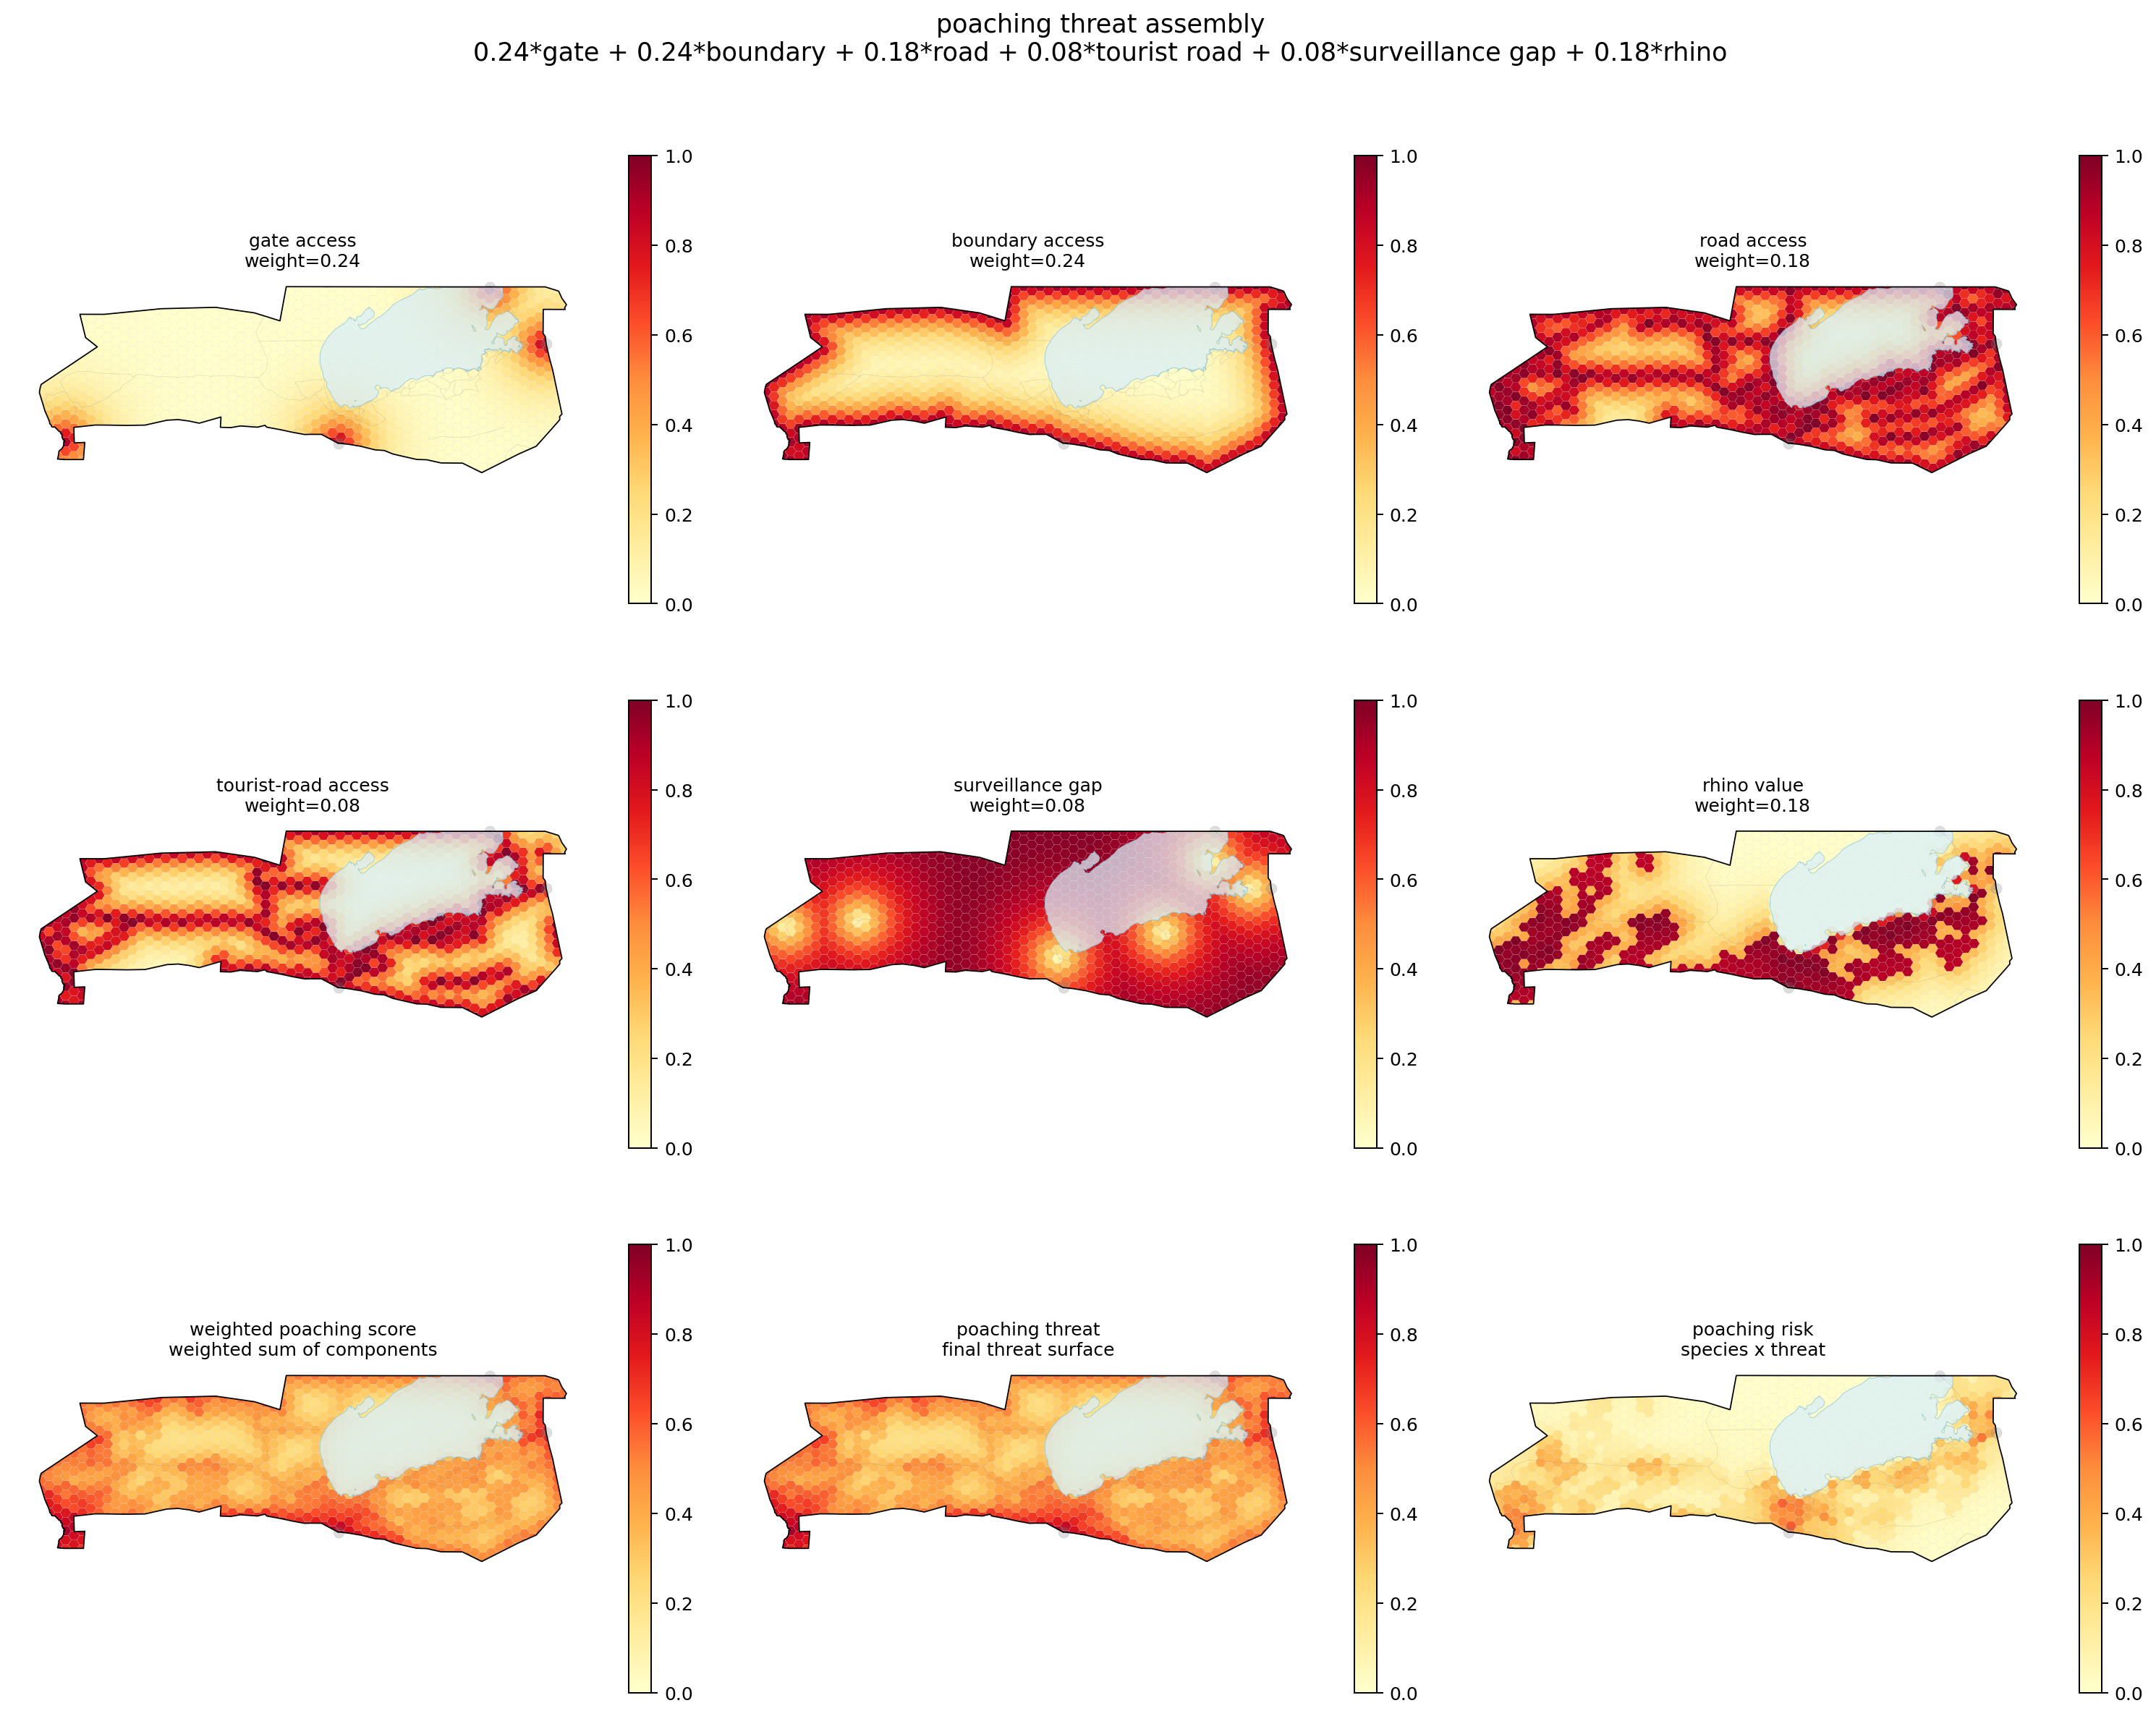
\includegraphics[width=0.95\textwidth]{risk_diagnostics/03_poaching_components.png}
\caption{Poaching-risk component layers and the resulting poaching threat surface. The panel set makes the weighted construction of $P_i$ visible by showing the underlying access, surveillance, and rhino-value terms on the common hex grid.}
\label{fig:risk_poaching_components}
\end{figure}
\subsection{Wildfire Risk}
For wildfire, the threat layer is based on three factors: whether the land is flammable, how far it is from water, and whether there has already been a recent fire event. The wildfire score is
\[
W_i
=
\bigl(0.60\,F_i + 0.40\,M_i\bigr)\,H_i,
\]
where $F_i$ is flammable land, $M_i$ is water remoteness, and $H_i$ is the recent-fire suppression factor. This means wildfire risk is highest in hexagons with burnable land, limited nearby water, and no recent fire event that would reduce fuel. The fuel-limitation and moisture-proximity factors follow established drivers of burnt area in Southern African savannas \cite{archibald2009fire}.

\begin{figure}[H]
\centering
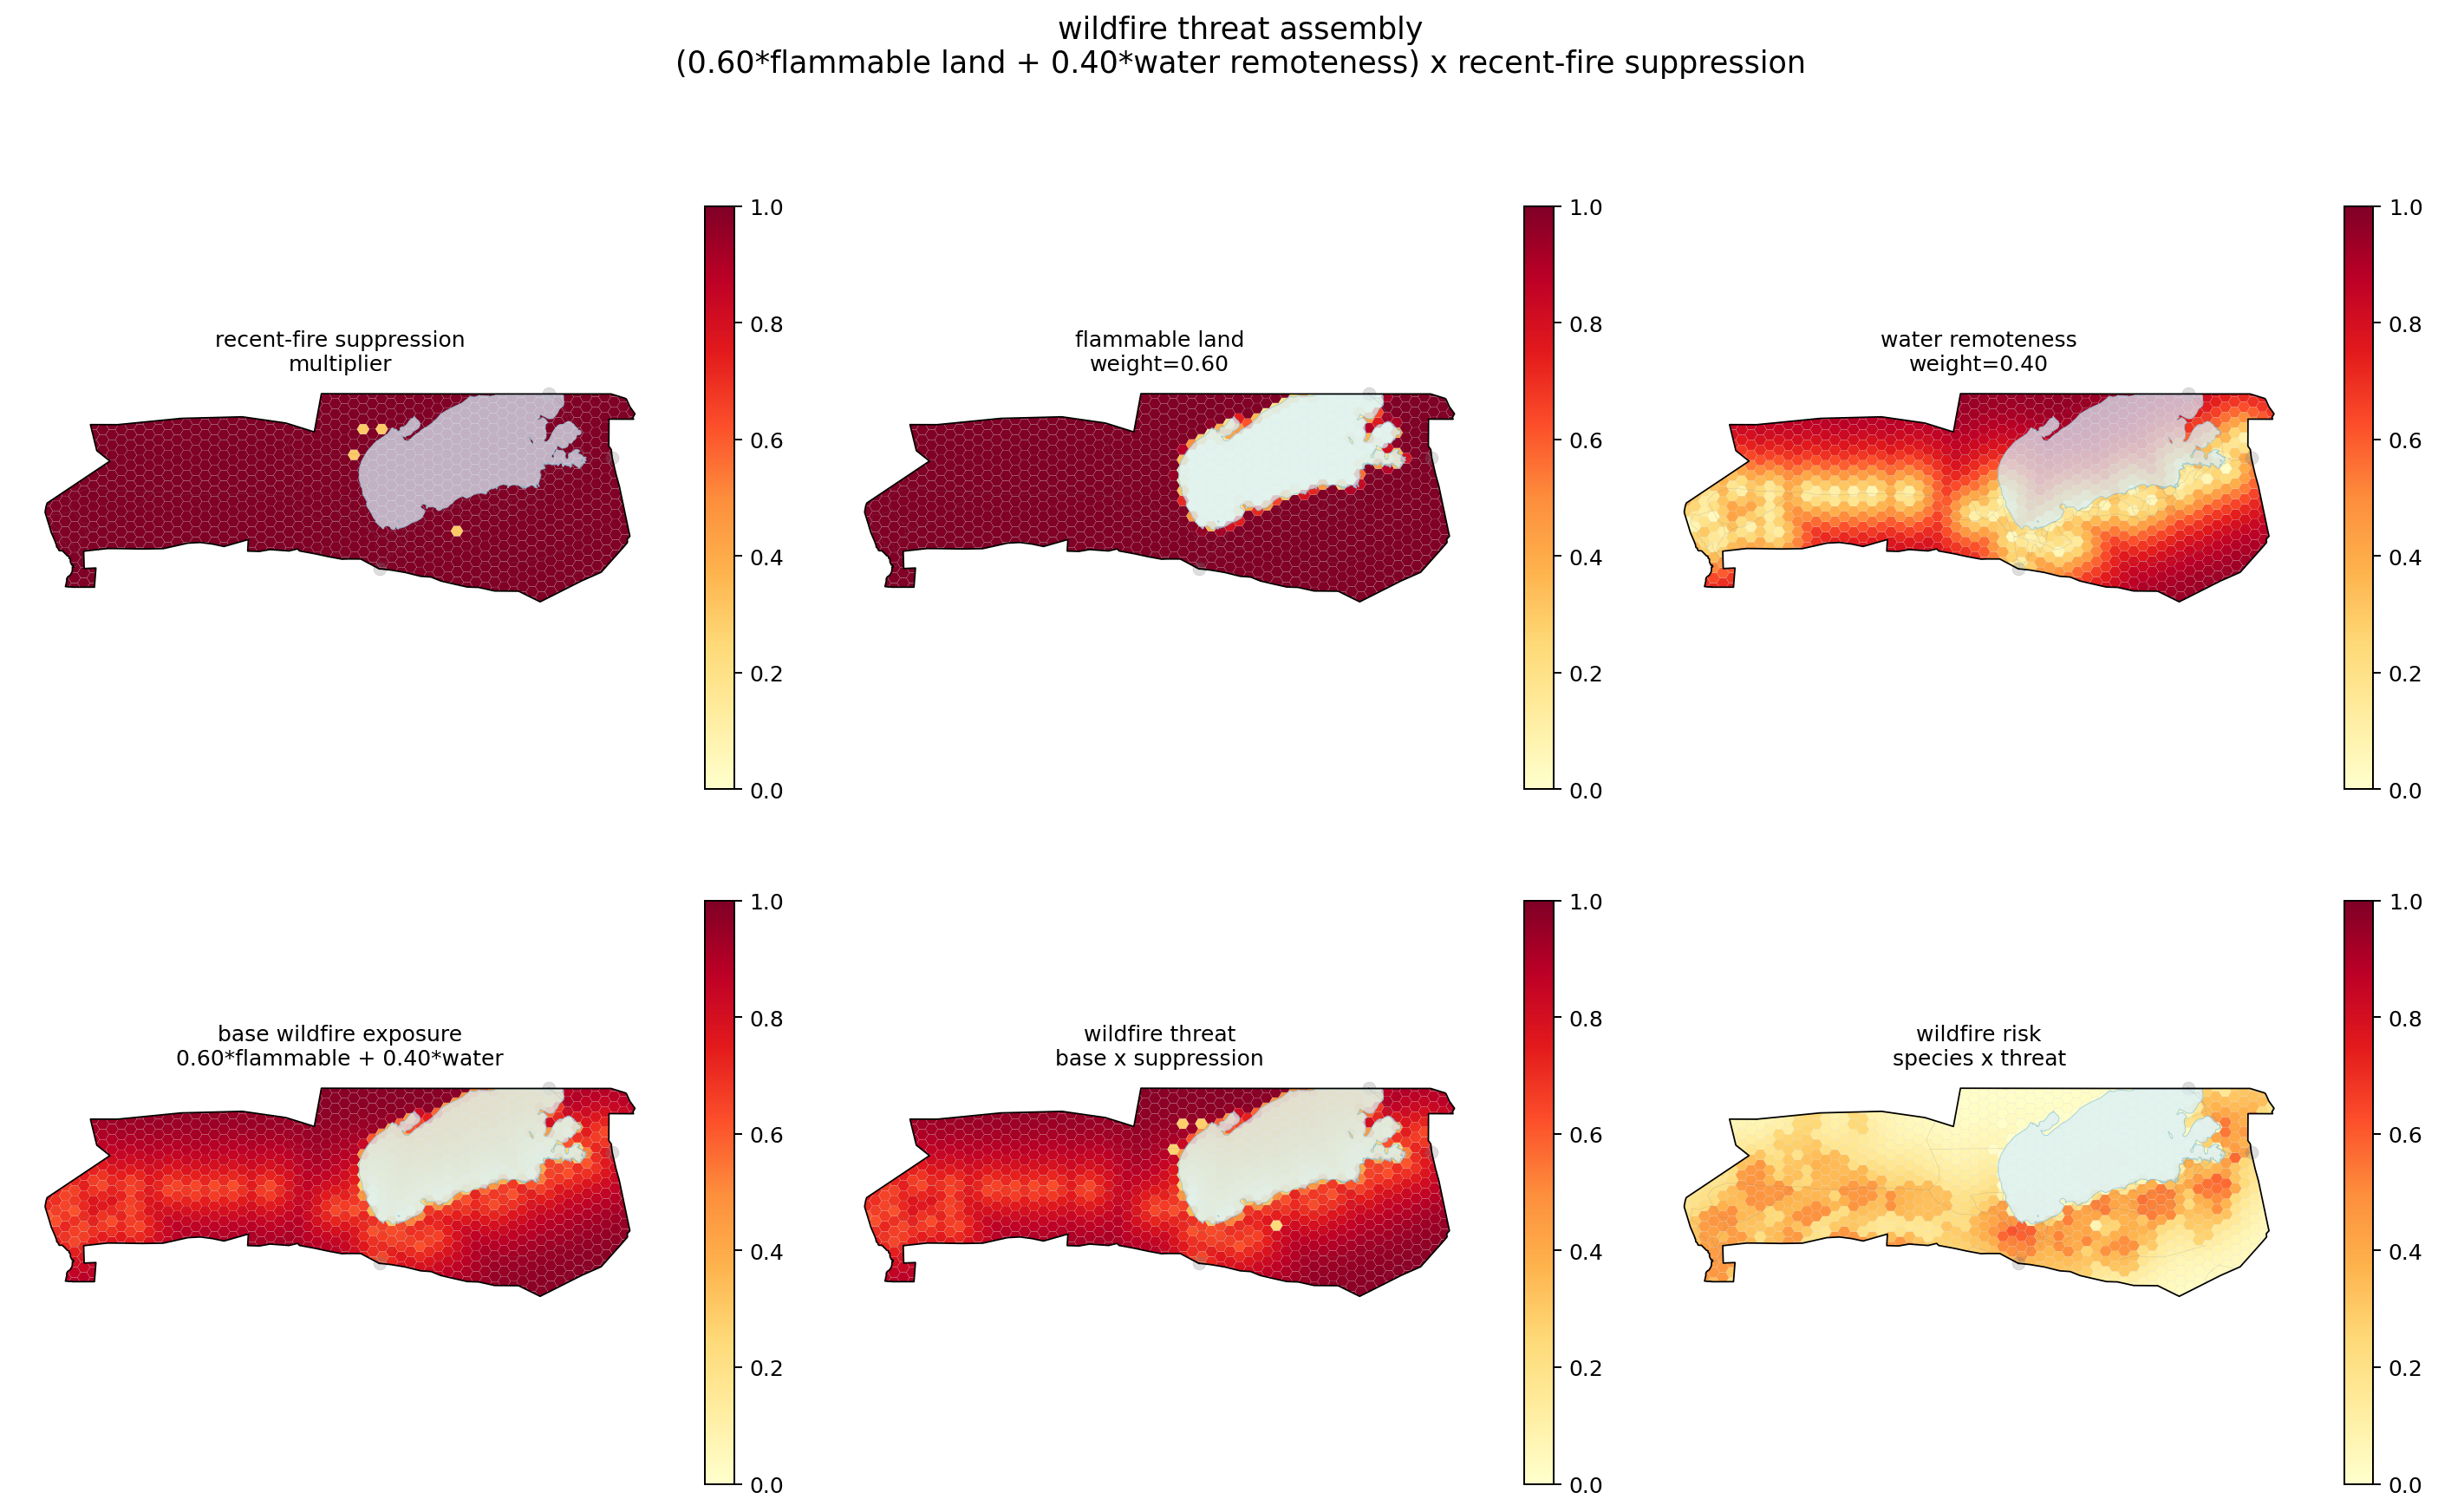
\includegraphics[width=0.95\textwidth]{risk_diagnostics/04_wildfire_components.png}
\caption{Wildfire-risk component layers and the resulting wildfire threat surface. The figure shows how flammability, water remoteness, and recent-fire suppression combine to produce the landscape-scale wildfire score $W_i$.}
\label{fig:risk_wildfire_components}
\end{figure}

\subsection{Tourism Risk}
For tourism, we first build a pressure layer from access to tourist roads, camps, gates, and waterholes:
\[
U_i
=
0.35\,R_i^{\mathrm{tour}}
+
0.25\,C_i
+
0.15\,G_i
+
0.25\,W_i^{\mathrm{hole}},
\]
where $R_i^{\mathrm{tour}}$ is tourist-road access, $C_i$ is camp access, $G_i$ is gate access, and $W_i^{\mathrm{hole}}$ is waterhole access. We then combine this pressure with wildlife presence:
\[
L_i
=
0.45\,E_i
+
0.25\,L_i^{\mathrm{lion}}
+
0.30\,H_i^{\mathrm{herb}},
\]
and define tourism threat by
\[
T_i = U_i \cdot L_i.
\]
This means tourism risk depends not only on where tourists can go, but also on where tourists and wildlife are likely to overlap \cite{newsome2012tourism}.

\begin{figure}[H]
\centering
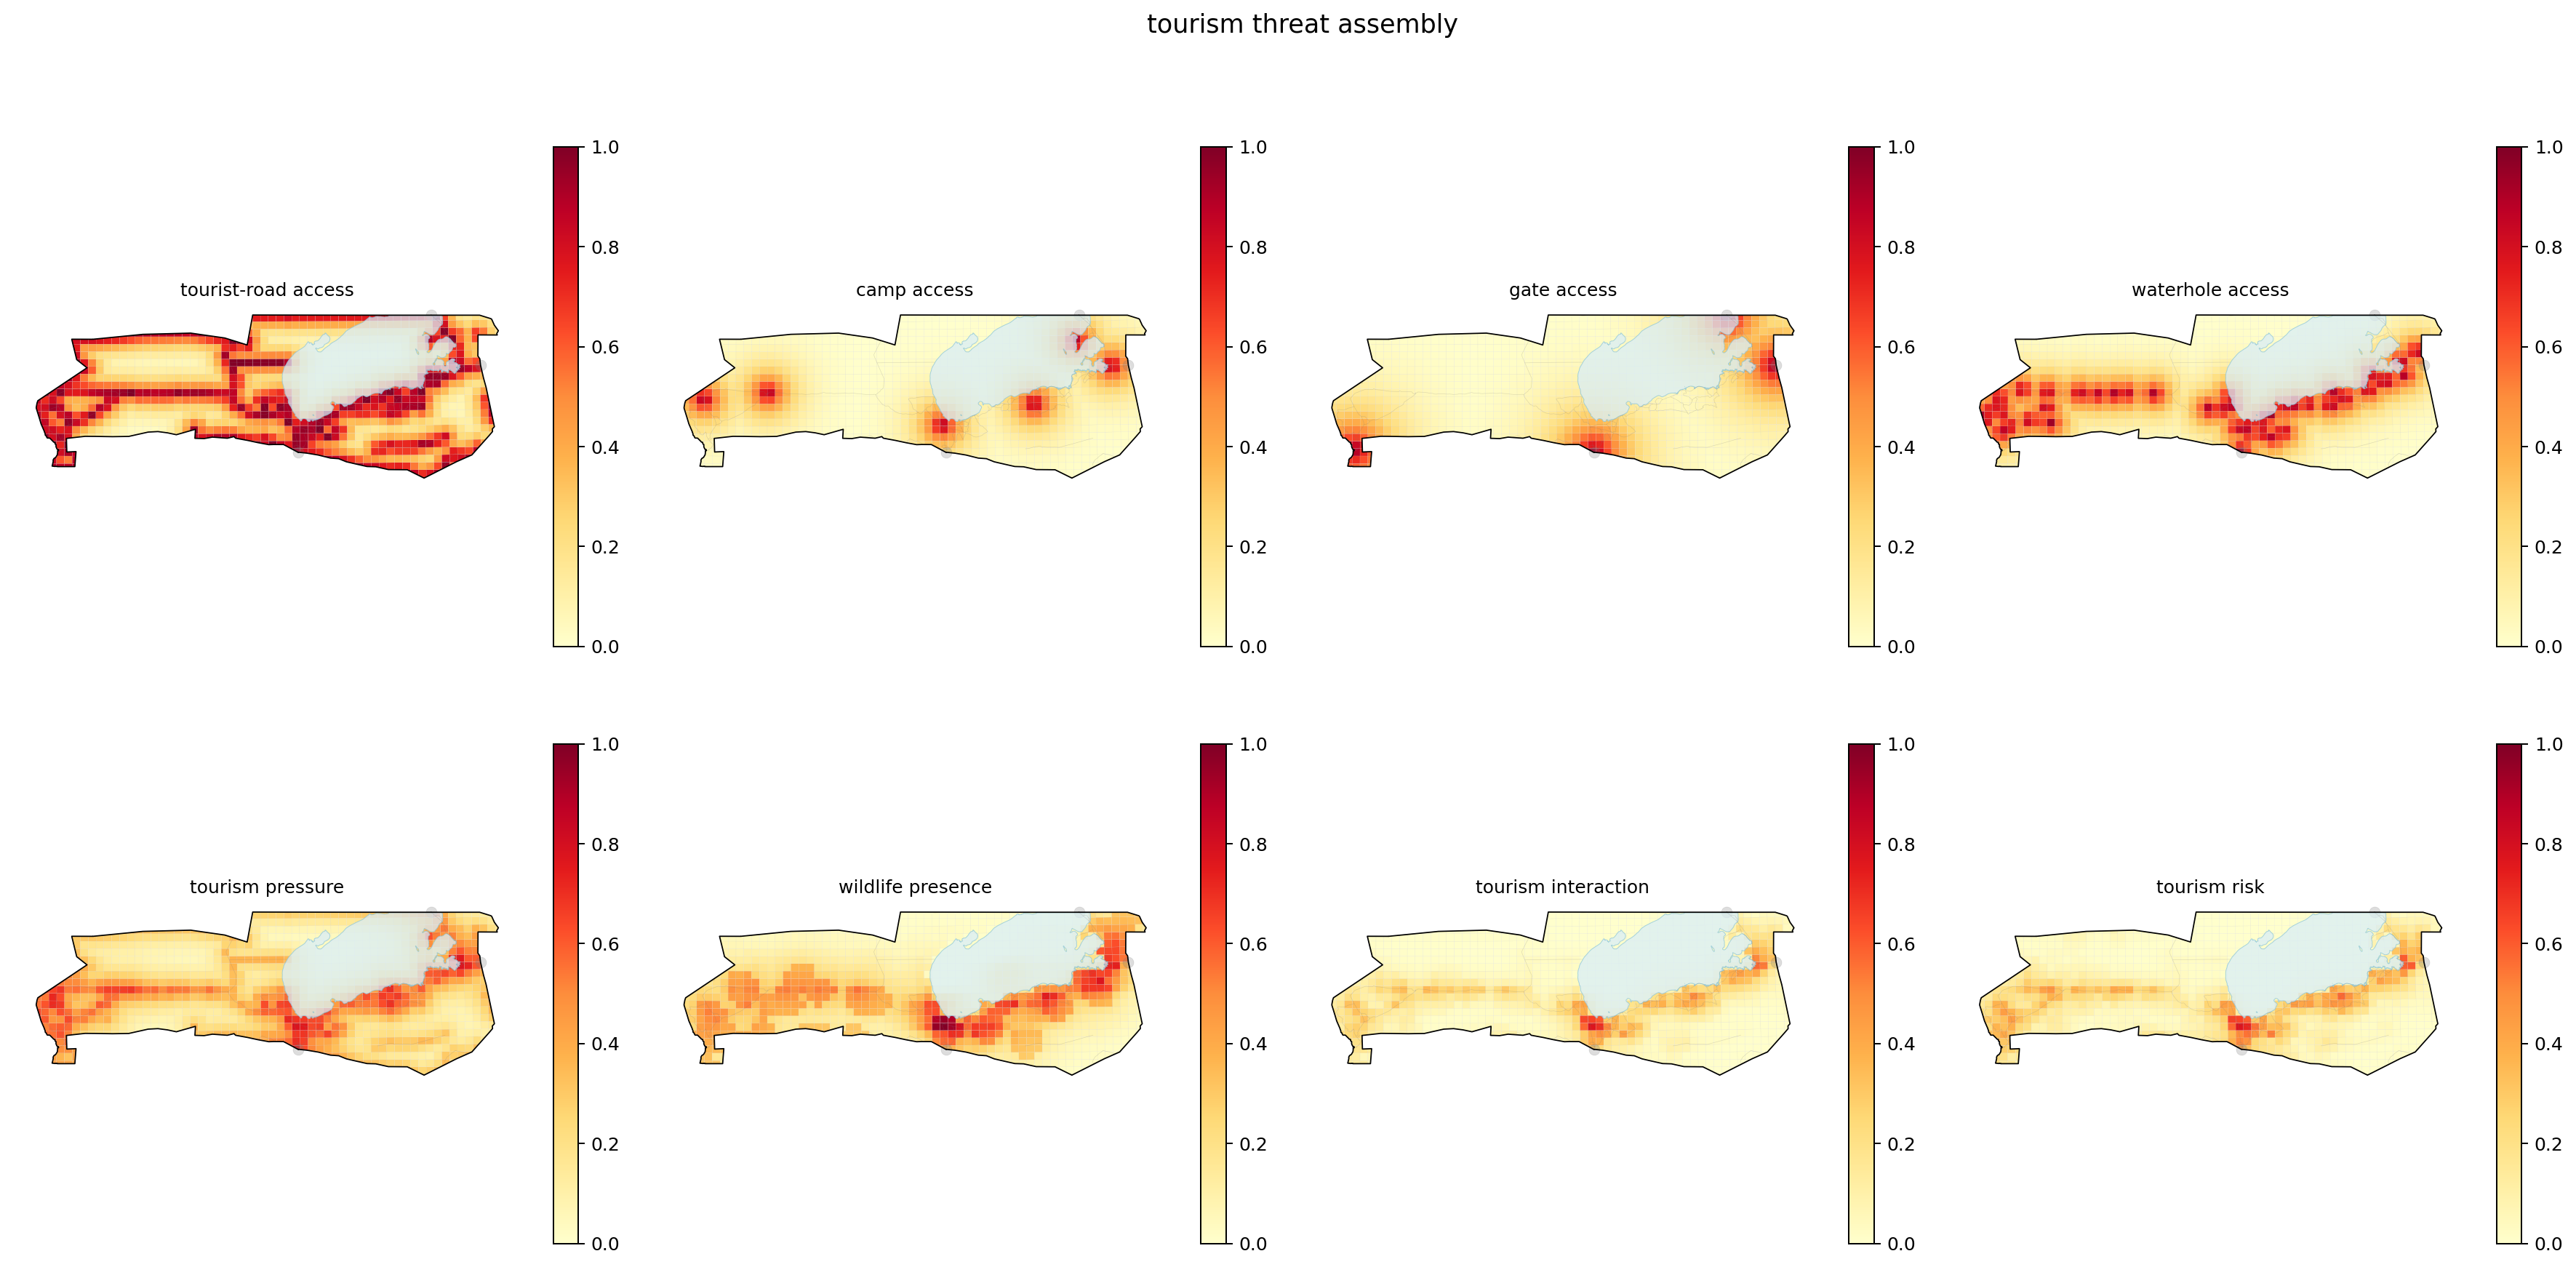
\includegraphics[width=0.95\textwidth]{risk_diagnostics/05_tourism_components.png}
\caption{Tourism-risk component layers and the resulting tourism threat surface. These panels show the access-pressure terms, wildlife-overlap terms, and the final tourism score generated from their interaction.}
\label{fig:risk_tourism_components}
\end{figure}

After building these threat layers, we combine them with the wildlife layers through a risk tensor. For each hexagon, each species value is multiplied by each threat value. If $x_{is}$ is the normalized support of species $s$ in hexagon $i$, and $y_{ik}$ is the normalized exposure of threat $k$ in hexagon $i$, then the tensor entry is
\[
R_{isk} = x_{is}\,y_{ik}.
\]
This gives a species-by-threat risk value for every hexagon. We then average across species to get one risk score per hexagon for each threat:
\[
R_{i}^{\mathrm{poach}} = \frac{1}{4}\sum_{s} R_{is,\mathrm{poach}},
\qquad
R_{i}^{\mathrm{fire}} = \frac{1}{4}\sum_{s} R_{is,\mathrm{fire}},
\qquad
R_{i}^{\mathrm{tour}} = \frac{1}{4}\sum_{s} R_{is,\mathrm{tour}}.
\]
\subsection{Total Risk}

Finally, we compute composite risk as a weighted average of the three threat-specific layers. The weights are
\[
w_{\mathrm{poach}} = 1.0,
\qquad
w_{\mathrm{fire}} = 1.5,
\qquad
w_{\mathrm{tour}} = 0.5.
\]
Thus the composite score in hexagon $i$ is
\[
R_i^{\mathrm{comp}}
=
\frac{
1.0\,R_i^{\mathrm{poach}}
+
1.5\,R_i^{\mathrm{fire}}
+
0.5\,R_i^{\mathrm{tour}}
}{
1.0+1.5+0.5
}.
\]
We chose these weights so that wildfire contributes the most to the composite layer, poaching contributes at a medium level, and tourism contributes at a smaller but still visible level. This reflects the role of wildfire as a broader landscape-scale threat in the current model, while tourism risk remains more spatially concentrated.

\begin{figure}[H]
\centering
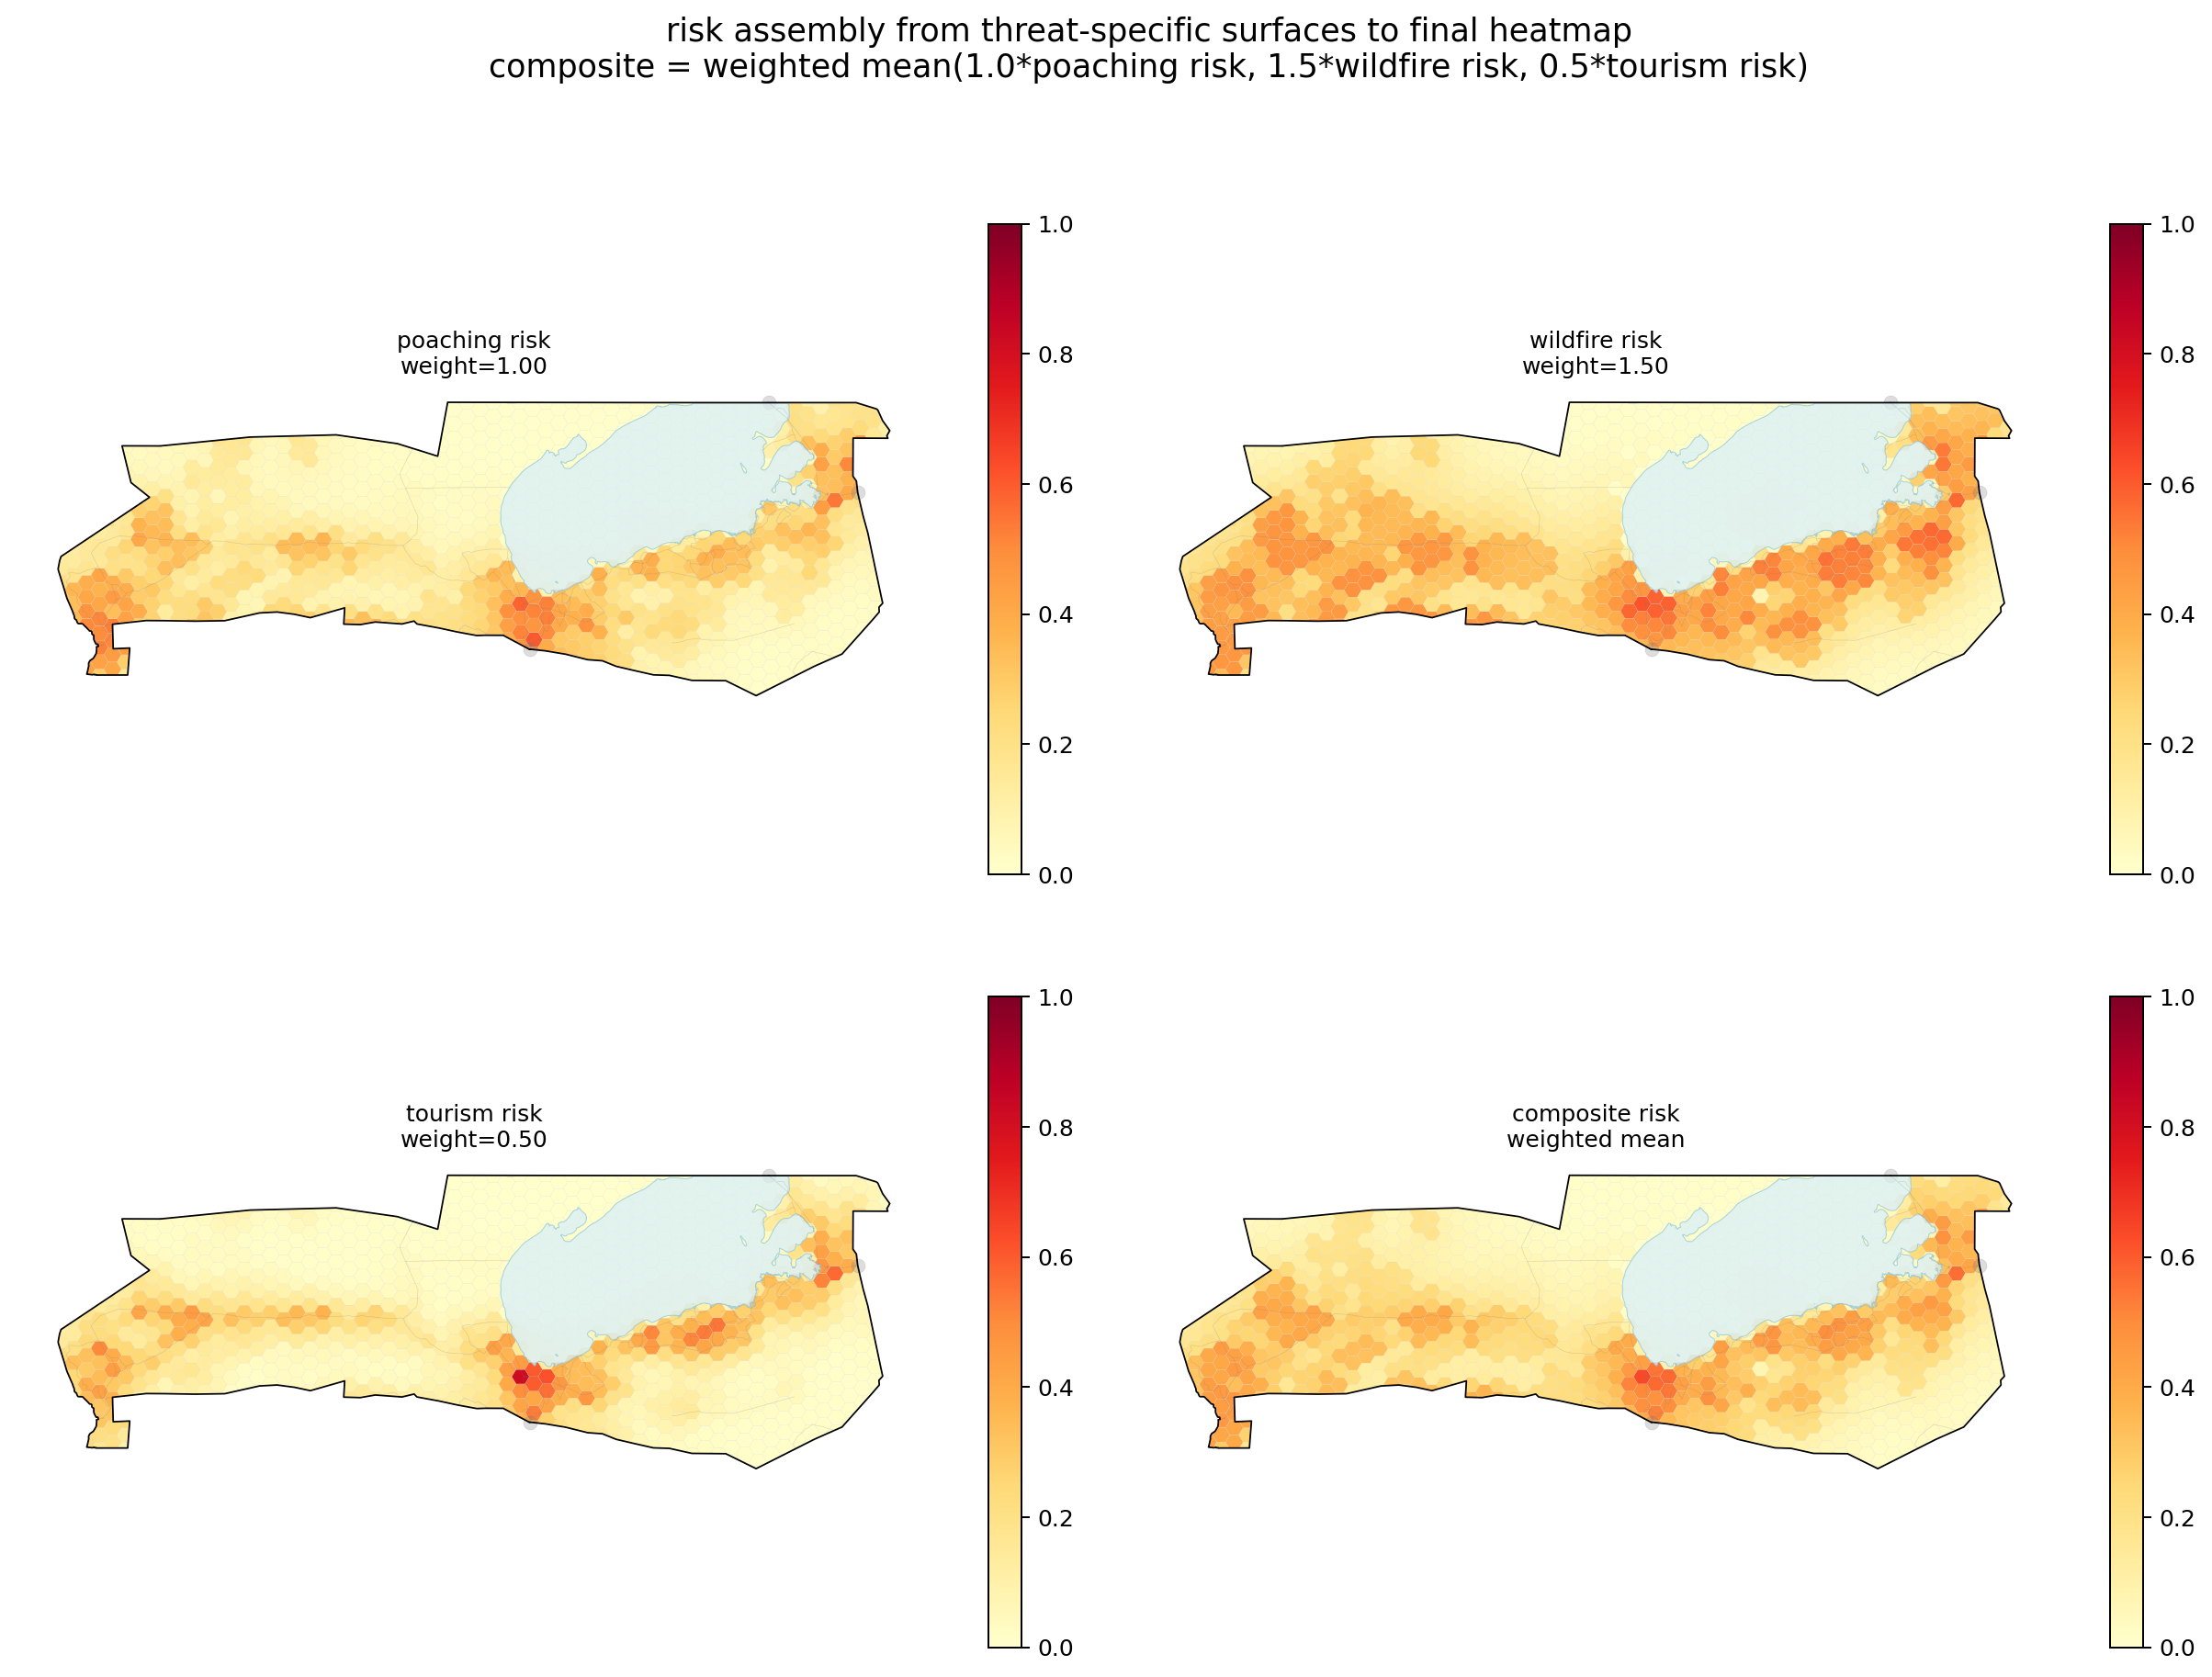
\includegraphics[width=0.95\textwidth]{risk_diagnostics/06_risk_assembly_overview.png}
\caption{Risk heat maps for Etosha National Park on a hexagonal grid. The four panels show composite risk, poaching risk, wildfire risk, and tourism risk on the same normalized scale from 0 to 1. Each hexagon combines wildlife support with threat exposure, allowing risk to be compared across the park using a consistent spatial unit. The composite layer combines the three threat-specific maps into one overall risk surface for later planning and resource allocation.}
\label{fig:risk_heat_maps}
\end{figure}

The final heat maps show that risk is not evenly distributed across Etosha. Poaching risk is concentrated in more accessible areas with stronger rhino support. Wildfire risk is more spread out across the park. Tourism risk is the most localized of the three layers. The composite map brings these patterns together into one planning surface, which is then used in the next stage of the model for surveillance and response decisions.
